\let\negmedspace\undefined 
 \let\negthickspace\undefined 
\documentclass[journal,12pt,onecolumn]{IEEEtran} 
 %\documentclass[conference]{IEEEtran} 
 %\IEEEoverridecommandlockouts 
 % The preceding line is only needed to identify funding in the first footnote. If that is unneeded, please comment it out. 
 \usepackage{cite} 
 \usepackage{amsmath,amssymb,amsfonts,amsthm} 
 \usepackage{algorithmic} 
 \usepackage{graphicx} 
 \usepackage{textcomp} 
 \usepackage{xcolor} 
 \usepackage{txfonts} 
 \usepackage{listings} 
 \usepackage{enumitem} 
 \usepackage{mathtools} 
 \usepackage{gensymb} 
 \usepackage[breaklinks=true]{hyperref} 
 \usepackage{tkz-euclide} % loads  TikZ and tkz-base 
 \usepackage{listings} 
 \usepackage{caption}
 % 
 %\usepackage{setspace} 
 %\usepackage{gensymb} 
 %\doublespacing 
 %\singlespacing 
  
 %\usepackage{graphicx} 
 %\usepackage{amssymb} 
 %\usepackage{relsize} 
  %\usepackage[cmex10]{amsmath} 
 %\usepackage{amsthm} 
 %\interdisplaylinepenalty=2500 
 %\savesymbol{iint} 
 %\usepackage{txfonts} 
 %\restoresymbol{TXF}{iint} 
 %\usepackage{wasysym} 
 %\usepackage{amsthm} 
 %\usepackage{iithtlc} 
 %\usepackage{mathrsfs} 
 %\usepackage{txfonts} 
 %\usepackage{stfloats} 
 %\usepackage{bm} 
 %\usepackage{cite} 
 %\usepackage{cases} 
 %\usepackage{subfig} 
 %\usepackage{xtab} 
 %\usepackage{longtable} 
 %\usepackage{multirow} 
 %\usepackage{algorithm} 
 %\usepackage{algpseudocode} 
 %\usepackage{enumitem} 
 %\usepackage{mathtools} 
 %\usepackage{tikz} 
 %\usepackage{circuitikz} 
 %\usepackage{verbatim} 
 %\usepackage{tfrupee} 
 %\usepackage{stmaryrd} 
 %\usetkzobj{all} 
 %    \usepackage{color}                                            %% 
 %    \usepackage{array}                                            %% 
 %    \usepackage{longtable}                                        %% 
 %    \usepackage{calc}                                             %% 
 %    \usepackage{multirow}                                         %% 
 %    \usepackage{hhline}                                           %% 
 %    \usepackage{ifthen}                                           %% 
   %optionally (for landscape tables embedded in another document): %% 
 %    \usepackage{lscape}      
 %\usepackage{multicol} 
 %\usepackage{chngcntr} 
 %\usepackage{enumerate} 
  
 %\usepackage{wasysym} 
 %\newcounter{MYtempeqncnt} 
 \DeclareMathOperator*{\Res}{Res} 
 %\renewcommand{\baselinestretch}{2} 
 \renewcommand\thesection{\arabic{section}} 
 \renewcommand\thesubsection{\thesection.\arabic{subsection}} 
 \renewcommand\thesubsubsection{\thesubsection.\arabic{subsubsection}} 
  
 \renewcommand\thesectiondis{\arabic{section}} 
 \renewcommand\thesubsectiondis{\thesectiondis.\arabic{subsection}} 
 \renewcommand\thesubsubsectiondis{\thesubsectiondis.\arabic{subsubsection}} 
  
 % correct bad hyphenation here 
 \hyphenation{op-tical net-works semi-conduc-tor} 
 \def\inputGnumericTable{}                                 %% 
  
 \lstset{ 
 %language=C, 
 frame=single,  
 breaklines=true, 
 columns=fullflexible 
 } 
 %\lstset{ 
 %language=tex, 
 %frame=single,  
 %breaklines=true 
 %} 
  
 \begin{document} 
 % 
  
  
 \newtheorem{theorem}{Theorem}[section] 
 \newtheorem{problem}{Problem} 
 \newtheorem{proposition}{Proposition}[section] 
 \newtheorem{lemma}{Lemma}[section] 
 \newtheorem{corollary}[theorem]{Corollary} 
 \newtheorem{example}{Example}[section] 
 \newtheorem{definition}[problem]{Definition} 
 %\newtheorem{thm}{Theorem}[section]  
 %\newtheorem{defn}[thm]{Definition} 
 %\newtheorem{algorithm}{Algorithm}[section] 
 %\newtheorem{cor}{Corollary} 
 \newcommand{\BEQA}{\begin{eqnarray}} 
 \newcommand{\EEQA}{\end{eqnarray}} 
 \newcommand{\define}{\stackrel{\triangle}{=}} 
  
 \bibliographystyle{IEEEtran} 
 %\bibliographystyle{ieeetr} 
  
  
 \providecommand{\mbf}{\mathbf} 
 \providecommand{\pr}[1]{\ensuremath{\Pr\left(#1\right)}} 
 \providecommand{\qfunc}[1]{\ensuremath{Q\left(#1\right)}} 
 \providecommand{\sbrak}[1]{\ensuremath{{}\left[#1\right]}} 
 \providecommand{\lsbrak}[1]{\ensuremath{{}\left[#1\right]}} 
 \providecommand{\rsbrak}[1]{\ensuremath{{}\left[#1\right]}} 
 \providecommand{\brak}[1]{\ensuremath{\left(#1\right)}} 
 \providecommand{\lbrak}[1]{\ensuremath{\left(#1\right.}} 
 \providecommand{\rbrak}[1]{\ensuremath{\left.#1\right)}} 
 \providecommand{\cbrak}[1]{\ensuremath{\left\{#1\right\}}} 
 \providecommand{\lcbrak}[1]{\ensuremath{\left\{#1\right.}} 
 \providecommand{\rcbrak}[1]{\ensuremath{\left.#1\right\}}} 
 \theoremstyle{remark} 
 \newtheorem{rem}{Remark} 
 \newcommand{\sgn}{\mathop{\mathrm{sgn}}} 
 \providecommand{\abs}[1]{\left\vert#1\right\vert} 
 \providecommand{\res}[1]{\Res\displaylimits_{#1}}  
 \providecommand{\norm}[1]{\left\lVert#1\right\rVert} 
 %\providecommand{\norm}[1]{\lVert#1\rVert} 
 \providecommand{\mtx}[1]{\mathbf{#1}} 
 \providecommand{\mean}[1]{E\left[ #1 \right]} 
 \providecommand{\fourier}{\overset{\mathcal{F}}{ \rightleftharpoons}} 
 %\providecommand{\hilbert}{\overset{\mathcal{H}}{ \rightleftharpoons}} 
 \providecommand{\system}{\overset{\mathcal{H}}{ \longleftrightarrow}} 
         %\newcommand{\solution}[2]{\textbf{Solution:}{#1}} 
 \newcommand{\solution}{\noindent \textbf{Solution: }} 
 \newcommand{\cosec}{\,\text{cosec}\,} 
 \providecommand{\dec}[2]{\ensuremath{\overset{#1}{\underset{#2}{\gtrless}}}} 
 \newcommand{\myvec}[1]{\ensuremath{\begin{pmatrix}#1\end{pmatrix}}} 
 \newcommand{\mydet}[1]{\ensuremath{\begin{vmatrix}#1\end{vmatrix}}} 
 %\numberwithin{equation}{section} 
 %\numberwithin{equation}{subsection} 
 %\numberwithin{problem}{section} 
 %\numberwithin{definition}{section} 
 %\makeatletter 
 %\@addtoreset{figure}{problem} 
 %\makeatother 
  
 %\let\StandardTheFigure\thefigure 
 \let\vec\mathbf 
 %\renewcommand{\thefigure}{\theproblem.\arabic{figure}} 
 %\renewcommand{\thefigure}{\theproblem} 
 %\setlist[enumerate,1]{before=\renewcommand\theequation{\theenumi.\arabic{equation}} 
 %\counterwithin{equation}{enumi} 
  
  
 %\renewcommand{\theequation}{\arabic{subsection}.\arabic{equation}} 
  
 %\def\putbox#1#2#3{\makebox[0in][l]{\makebox[#1][l]{}\raisebox{\baselineskip}[0in][0in]{\raisebox{#2}[0in][0in]{#3}}}} 
 %     \def\rightbox#1{\makebox[0in][r]{#1}} 
 %     \def\centbox#1{\makebox[0in]{#1}} 
 %     \def\topbox#1{\raisebox{-\baselineskip}[0in][0in]{#1}} 
 %     \def\midbox#1{\raisebox{-0.5\baselineskip}[0in][0in]{#1}} 
  
 \vspace{3cm} 
  
 \title{ Hardwware Assignment  
  
         \Large AI1110: Probability and Random Variables 
 } 
 \author{ Dhana Lakshmi
          
         AI22BTECH11012 
 } 
  
 \maketitle 
  
 \bigskip 
 \renewcommand{\thefigure}{\theenumi} 
 \renewcommand{\thetable}{\theenumi} 
 
 \begin{enumerate}[label=(\alph*)] 
 \item Description : 
 The random number generator project explores the utilization of an IC555 timer circuit with an XOR gate to generate random numbers.7-segment displays provide a convenient way of displaying numbers from zero to nine as they basically consist of a load of light emitting diodes connected together within a single indicator package.The circuit uses 5V from Micro USB and this is Vcc for the circuit.
 \item Components : 
%%%%%%%%%%%%%%%%%%%%%%%%%%%%%%%%%%%%%%%%%%%%%%%%%%%%%%%%%%%%%%%%%%%%%%
%%                                                                  %%
%%  This is a LaTeX2e table fragment exported from Gnumeric.        %%
%%                                                                  %%
%%%%%%%%%%%%%%%%%%%%%%%%%%%%%%%%%%%%%%%%%%%%%%%%%%%%%%%%%%%%%%%%%%%%%%
 \begin{table}[htpb]
\centering 
\caption{Components}
\label{tab:components}
%%%%%%%%%%%%%%%%%%%%%%%%%%%%%%%%%%%%%%%%%%%%%%%%%%%%%%%%%%%%%%%%%%%%%%
%%                                                                  %%
%%  This is a LaTeX2e table fragment exported from Gnumeric.        %%
%%                                                                  %%
%%%%%%%%%%%%%%%%%%%%%%%%%%%%%%%%%%%%%%%%%%%%%%%%%%%%%%%%%%%%%%%%%%%%%%
\begin{tabular}{|c|c|c|}
\hline
Component		&Value	 	&Quantity\\
\hline
Breadboard		&	&1\\
\hline
Seven Segment Display			&Common Anode	&1\\
\hline
Decoder		&7447		&1\\
\hline
Flip Flop	&7474		&2\\
\hline
X-OR GATE		&7486		&1\\
\hline
555 IC	&		&1\\
\hline
Resistor		&1K\$$\backslash$Omega\$	&1\\
\hline
Resistor		&1M\$$\backslash$Omega\$		&1\\
\hline
Capacitor		&100nF		&1\\
\hline
Capacitor		&10nF		&1\\
\hline
Jumper Wires	&			&20\\
\hline
\end{tabular}

\end{table}

\item Observation : 
\setcounter{enumi}{3}
The XOR gate introduces randomness by XORing the signals from the IC555 timer circuit. 
The resistor and capacitors influence the timing and stability of the circuit, affecting the randomness of the generated numbers.  
The displayer effectively presents the random numbers produced by the circuit.

\item Block Diagram and Image of Circuit : 
  \begin{figure}[ht]
    \centering
    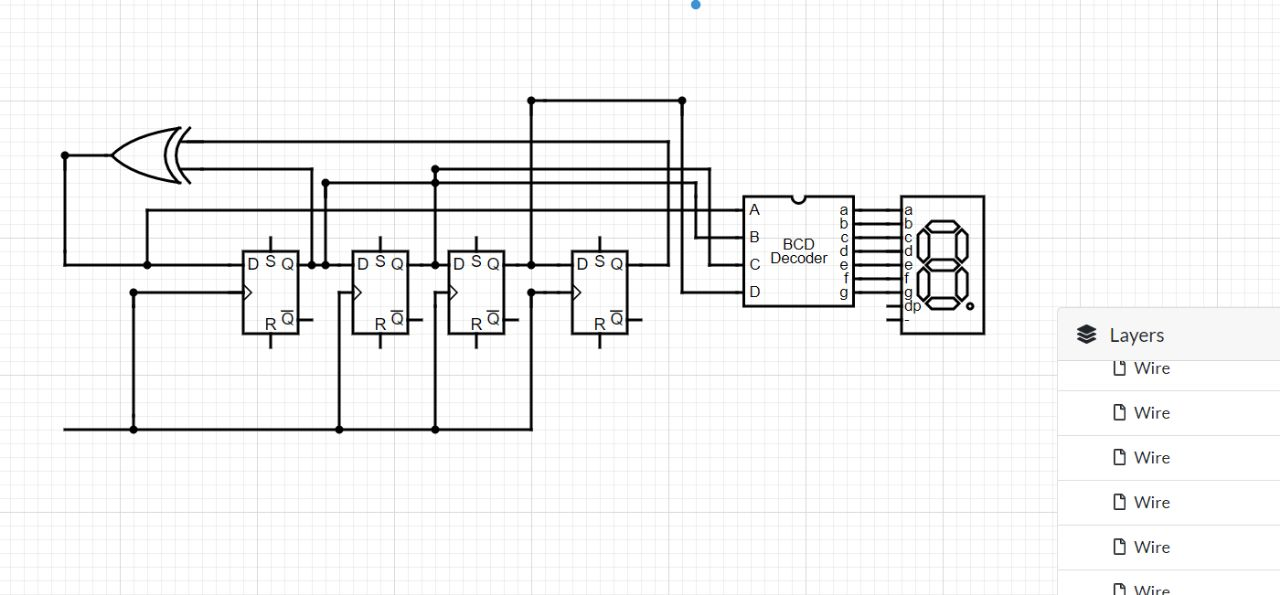
\includegraphics[width=0.7\linewidth]{pictures/img.jpeg}
    \caption{Block Diagram}
    \label{fig:img}
  \end{figure}
  \begin{figure}[ht]
   \centering
   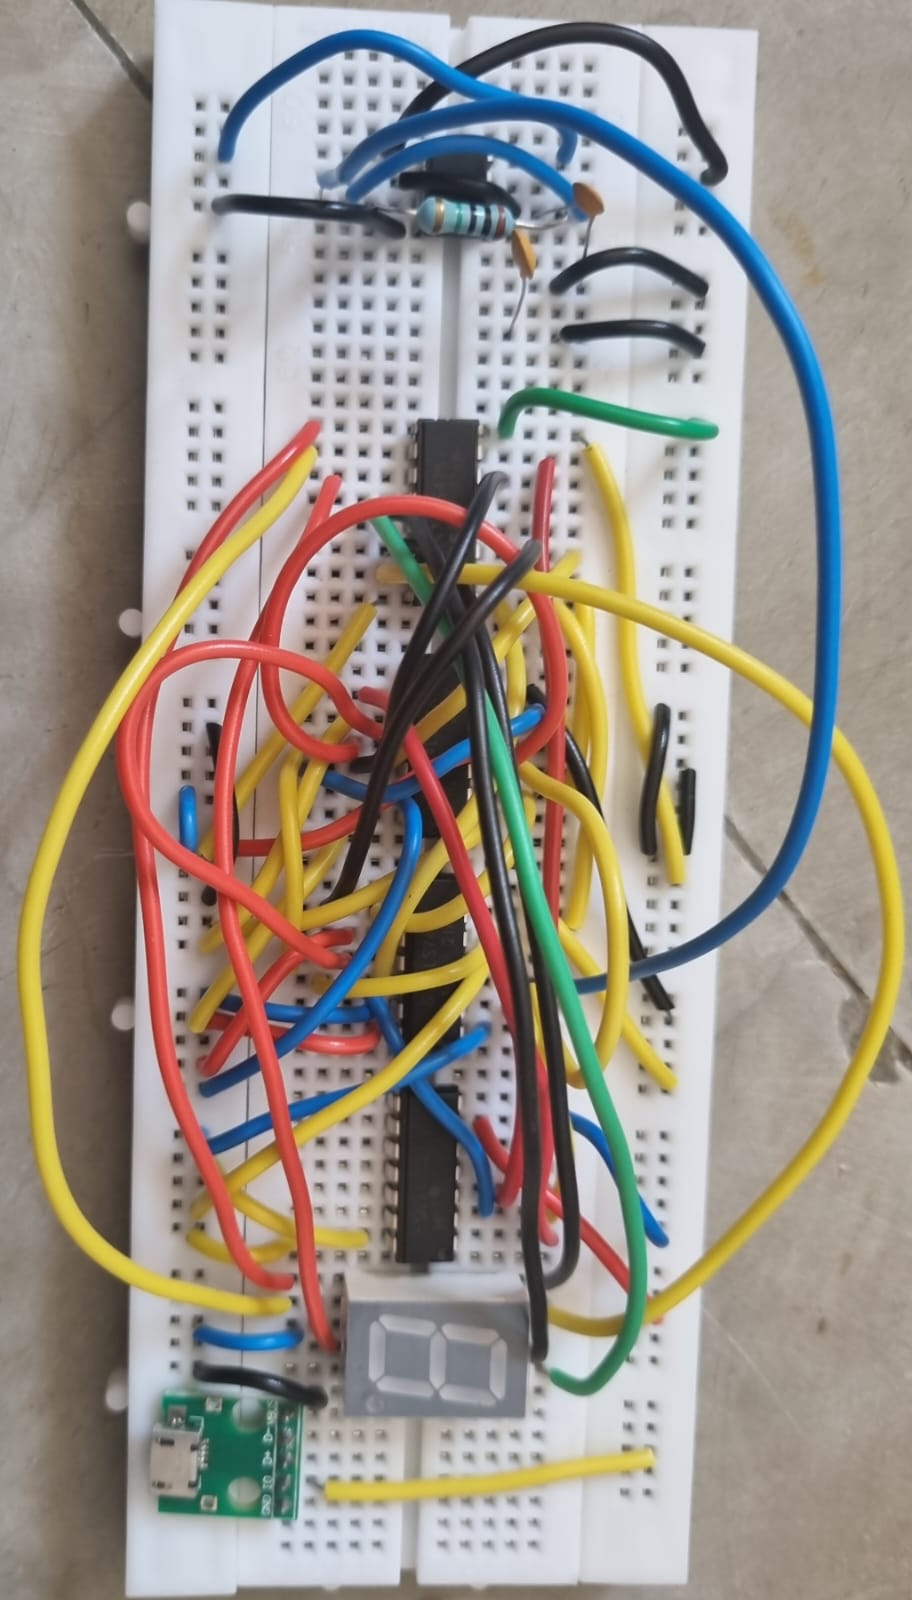
\includegraphics[width=0.7\linewidth]{pictures/img1.jpeg}
   \caption{Image of Circuit}
   \label{fig:img1}
   \end{figure}

\end{enumerate} 
 \end{document}
